\chapter{Transformer Networks}
\label{ch-transformer}

This chapter in based on Refs.\cite{joshi-trans}
and \cite{wiki-transformer}.

Transformer Networks (TN)
have been taking the field of
Natural Language Processing (NLP)
by storm in recent years.
They were introduced in 2017 and already
are the basis of
BERT (Bidirectional Encoder
Representations from Transformers)
and GPT (Generative Pre-trained Transformer),
two TN libraries that
have been trained with
huge databases such as all of
English Wikipedia (2,500M words).

Recurrent Neural Nets (RNNs)
are discussed in Chapter \ref{ch-rnn}.
TNs are quickly displacing RNNs, 
an older method, in NLP.  TNs are better than RNNs 
for doing NLP in several important ways. Whereas
 RNNs analyze the tokens (words) of a sentence 
sequentially (like a Kalman Filter), 
TNs analyze them in parallel, and thus are more
 amenable to parallel computing. Also, because
 RNNs analyze the words of a sentence sequentially, 
they tend to give more importance to the end 
of a sentence than to its beginning. That's because 
RNNs start forgetting the beginning of a sentence
 by the time they reach its end, like a patient 
with Alzheimer's. TNs do not suffer from this malady.

Dynamical bnets are discussed in Chapter \ref{ch-dyn-bnet}.
In Chapter \ref{ch-rnn},
we showed that RNNs
are dynamical bnets.
The goal of
this chapter
is to define TNs,
and to show that they too are
dynamical bnets.

Let

$\cals$ be the
set of words in a sentence,

$x_i^t\in \RR^{nx}$ be
an $nx$ dimensional column vector
for word $i\in \cals$ at time $t$.

$W_\rvq^t, W_\rvk^t, W_\rvv^t\in \RR^{nx\times nx}$
be the  weight matrices for time
slice $t$.
These matrices are learned by training
the net.
The letters $Q,K,V$ stand for
 Query, Key and Value,
respectively.
They transform $x_i^t$ 
as follows

\beq
\left\{
\begin{array}{l}
v_i^t = W_\rvv^t x_i^t
\\
q_i^t = W_\rvq^t x_i^t
\\
k_i^t = W_\rvk^t x_i^t
\end{array}
\right.
\eeq



\begin{figure}[h!]
$$
\xymatrix@C=4pc{
&\rvv_0^t\ar[rrd]
\ar[rrdddd]\ar[rrddddddd]
\\
\rvx_0^t \ar[ru]^{W_{\rvv 0}^t}\ar@[red][r]^{W_{\rvq 0}^t}
\ar[rd]_{W_{\rvk 0}^t}
&\rvq_0^t\ar@[red][rr]
&&\rvx_0^{t+1}
\\
&\rvk_0^t\ar[rru]
\ar[rrdd]\ar[rrddddd]
\\
%%%%%
&\rvv_1^t\ar[rrd]
\ar[rrdddd]\ar[rruu]
\\
\rvx_1^t\ar[ru]^{W_{\rvv 1}^t}\ar@[red][r]^{W_{\rvq 1}^t}
\ar[rd]_{W_{\rvk 1}^t}
&\rvq_1^t\ar@[red][rr]
&&\rvx_1^{t+1}
\\
&\rvk_1^t\ar[rru]
\ar[rrdd]\ar[rruuuu]
\\
%%%%%
&\rvv_2^t\ar[rrd]
\ar[rruu]\ar[rruuuuu]
\\
\rvx_2^t \ar[ru]^{W_{\rvv 2}^t}\ar@[red][r]^{W_{\rvq 2}^t}\ar[rd]_{W_{\rvk 2}^t}
&\rvq_2^t\ar@[red][rr]
&&\rvx_2^{t+1}
\\
&\rvk_2^t\ar[rru]
\ar[rruuuu]\ar[rruuuuuuu]
}
$$
\caption{Time-slice $t$
of dynamical bnet for
 a transformer network (TN)
of a 3-word sentence.
Note that $k_i^t$
for all $i$
points to $\rvx^{t+1}_j$ for all $j$.
Likewise,
$\rvv_i^t$
for all $i$
points to $\rvx^{t+1}_j$ for all $j$.
However, 
$\rvq_i^t$
points only to $\rvx^{t+1}_i$.
}
\label{fig-transformer}
\end{figure}

Fig.\ref{fig-transformer}
represents a TN 
of a 3-word sentence as a dynamical bnet.
The TPMs,
printed in blue,
for bnet
Fig.\ref{fig-transformer},
are as follows:

\beq\color{blue}
P(v_i^t|W_\rvv^t, x_i^t)=
\indi(\;\;\;
v_i^t = W_\rvv^t x_i^t
\;\;\;)
\eeq

\beq\color{blue}
P(q_i^t|W_\rvq^t, x_i^t)=
\indi(\;\;\;
q_i^t = W_\rvq^t x_i^t
\;\;\;)
\eeq

\beq\color{blue}
P(k_i^t|W_\rvk^t, x_i^t)=
\indi(\;\;\;
k_i^t= W_\rvk^t x_i^t
\;\;\;)
\eeq

\beq\color{blue}
P(x^{t+1}_i|v_.^t,q_i^t,
 k_.^t)
=
\indi(\;\;\;
x_i^{t+1}=
\underbrace{
\sum_{j\in\cals}
v_j^t
\underbrace{
\frac{e^{(q_i^t)^T k_j^t}}
{\sum_{j'\in \cals}
e^{(q_i^t)^T k_{j'}^t}}
}_{w_{j|q_i^t}=
\softmax((q_i^t)^T k_j^t)(j)}\;
}_{E_{\rvj|q_i^t}[v_\rvj^t]={\bf Attention}}
\;\;\;)
\eeq


To improve stability
of the dynamical bnet,
it is common to think 
of the  matrices $W_\rvv^t, W_\rvq^t, W_\rvk^t$ as nodes
pointed to by a ``head" root node $\rvc
\in\{0,1, \ldots, nc-1\}$, with TPMs,
printed in blue, as follows.

\begin{subequations}
\beq\color{blue}
P(W_\rvv^t|c)=
\delta(W_\rvv^t, W_{\rvv c}^t)
\eeq

\beq\color{blue}
P(W_\rvq^t|c)=
\delta(W_\rvq^t, W_{\rvq c}^t)
\eeq

\beq\color{blue}
P(W_\rvk^t|c)=
\delta(W_\rvk^t, W_{\rvk c}^t)
\eeq
\end{subequations}
Even better,
one can go fully
Bayesian, 
and make
these 3  distributions 
arbitrary categorical
distributions  
to be determined by net training,
instead of mere
delta functions.

On first encounter, the structure of a Transformer net
seems a bit mysterious. Then one realizes that this is
an old friend. As shown in Fig.\ref{fig-transformer-TAN-Bayes}, if one 
shrinks some nodes
of the Transformer net, it becomes a TAN Bayes net. Each of the 3 subgraphs $\rvx^t, (\rvv^t, \rvq^t, \rvk^t), \rvx^{t+1} $
also constitutes a TAN Bayes net. (TAN Bayes nets
were introduced in Chapter \ref{ch-chow})\footnote{A {\bf reverse or upside down tree} is obtained by reversing the directions of all the arrows of a tree directed graph. A TAN Bayes net is normally defined as in Chapter\ref{ch-chow}, as a Naive Bayes net augmented with a tree. In transformers, the Naive Bayes Net is augmented with a reverse tree (RT) instead of a tree (T), so technically transformers contain RTAN (or simply AN) Bayes nets, not TAN Bayes nets. }

\begin{figure}[h!]
\centering
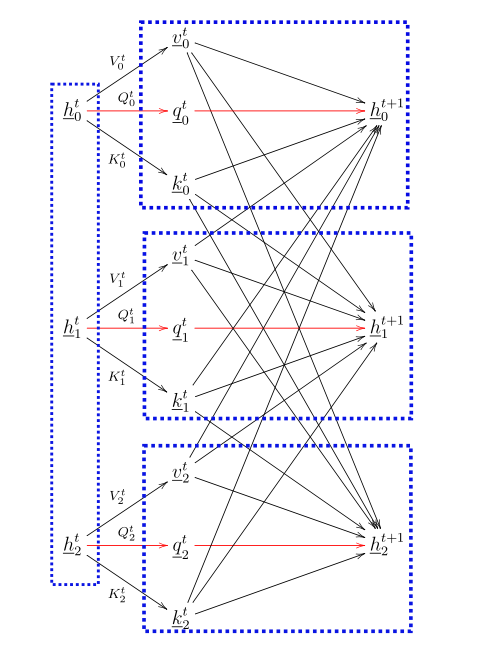
\includegraphics[width=3.5in]
{transformer/transformer-TAN-Bayes.png}
\caption{If the blue boxes in this graph are each ``shrunk" to single nodes,
then it becomes a TAN Bayes Net. Each of the 3 subgraphs $\rvx^t, (\rvv^t, \rvq^t, \rvk^t), \rvx^{t+1} $
also constitutes a TAN Bayes net. (TAN Bayes nets
were introduced in Chapter \ref{ch-chow}).}
\label{fig-transformer-TAN-Bayes}
\end{figure}

